\documentclass[UTF8]{article}
\usepackage{geometry}
\usepackage{amsmath}
\usepackage{amssymb}
\usepackage{listings}
\usepackage{xcolor}
\usepackage{graphicx}
\usepackage{float}
\usepackage[amssymb]{SIunits}

\geometry{a4paper,scale=0.72}
\setlength{\parindent}{0pt}

% Renew some basic command
\newcommand{\ds}{\displaystyle}
\newcommand{\dx}{\mathrm{d}x}
\newcommand{\dy}{\mathrm{d}y}
\newcommand{\ul}{\underline}

% Set indent
\setlength{\parindent}{1em}
\setlength{\parskip}{1.5ex}

\lstset{
    flexiblecolumns,
    numbers = left
}

\title{\bf DoA Estimation}
\author{Zike,Xu \ Zhiyi,Wang \ Dinghao,Cheng}
\date{\today}
\begin{document}
\maketitle
% Make 
\tableofcontents

\newpage
% \begin{abstract}
% \centering \small {{context}}
% \end{abstract}

\section{Narrowband Estimation}
\hspace{0.5em} We have obtained a stimulation data with $J = 4$ sensors in \emph{Observations\_nb.mat}, and we want to estimate angles of the source with MUSIC algorithm.

In MUSIC, there're some basic arguments, $J$ represents the number of sensors, and $P$ represents the number of sources ($P < J$).
The signal is given in the form of
\begin{equation}
    s(t) = A(t)e^{j\omega_c t + \phi(t)}
\end{equation}
when $A(t)$ is the envelop, $\phi(t)$ is the phase. In narrowband, they varies slow than $e^{j \omega_c t}$,
\begin{gather}
    s(t - \tau) = A(t - \tau) e^{j\omega_c(t - \tau)}e^{j\phi(t - \tau)} \approx A(t)e^{j\omega_c(t - \tau) \phi(t)} = e^{-j\omega_c\tau}\cdot s(t)
\end{gather}
thus, in narrowband, Time delay $\approx$ Phase shift.

Position J sensors on x-y axis, their relative position can be $p_i = (x, y)^t$. Consider just one far field signal passes the system with angle $\theta$(with y axis), which can be expressed as $\ul{v} = (\sin \theta, \cos \theta)^t$. The time delay of every sensors is $p v$. Convert it into phase shift, its $e^{-j 2 \pi \omega_c \Delta t}$, denote it as $a(\omega, \theta)$. Thus, we can construct a matrix with $a(\omega, \theta)$ which can shift the original signal as $\theta$ changes.
\begin{gather}
    s[k, \ul{p_i}] = s[k] \cdot e^{j \omega \tau_i} = s[k] \cdot a_i(\omega, \theta)
\end{gather}
For narrowband signal, we can acquire its $f_c$(center frequency) in advance, so $a_i(\omega, \theta)$ can be written as $a_i(\theta)$.

We model the system as
\begin{gather*}
    \ul{x}[k] = (x_1[k], x_2[k], x_3[k], \cdots, x_J[k])^t \\
    \ul{n}[k] = (n_1[k], n_2[k], n_3[k], \cdots, n_J[k])^t \\
    \ul{a}(\theta) = (a_1(\theta), a_2(\theta), a_3(\theta), \cdots, a_J(\theta))^t
\end{gather*}
in which 
\begin{gather}
    \ul{x}[k] = \ul{a}(\theta)\cdot s[k] + \ul{n}[k]
\end{gather}
for multiple sound sources, add them together to get
\begin{gather}
    x_i[k] = \sum_{p}a_i(\theta_p)\cdot s_p[k] + n_i[k] \Rightarrow \ul{x}[k] = A \cdot \ul{s}[k] + \ul{n}[k]
\end{gather}
A is a $J \times P$ matrix, and $\ul{s}[k]$ is the column vector consists of different sound sources.

Denoted the covariance matrix as $R_x$, 
\begin{gather}
   R_x = \mathbb{E}\{\ul{x}[k]\ul{x}^h[k]\} 
\end{gather}
expand it with $\ul{x}[k] = A \cdot \ul{s}[k] + \ul{n}[k]$, 
\begin{gather}
    \mathbb{E}\{\ul{x}[k]\ul{x}^h[k]\} = \mathbb{E} \{ (A \cdot \ul{s}[k] + \ul{n}[k])(A \cdot \ul{s}[k] + \ul{n}[k])^h \} \Rightarrow A \mathbb{E}\{ \ul{s}[k]\ul{s}^h[k] \}A^h + \mathbb{E}\{ \ul{n}[k] \ul{n}^h[k]\}
\end{gather}
$R_s = \mathbb{E}\{ \ul{s}[k]\ul{s}^h[k] \}$ is a Hermite positive definite matrix, so 
\begin{gather*}
    rank(R_s) = rank(A) = rank(A R_s A^h) = P_{source}
\end{gather*}
The rank of the matrix equals to its number of non-zero eigenvalues, so $A R_s A^h$ contains $J - P$ zero eigenvalues. 

Let $\ul{u_i}$ be the eigenvector corresponding to zero eigenvalues, so 
\begin{gather}
    \ul{u}_i^h A R_s A^h \ul{u}_i = \ul{0} \Rightarrow (A^h\ul{u}_i)^h R_s (A^h \ul{u}_i) = \ul{0} \Rightarrow A^h\ul{u}_i = \ul{0}
\end{gather}
Which claim that the $J - P$ zero eigenvectors is orthogonal to those steering vectors.

We traverse $\theta$ to get the minimal $\sum_{i}\ul{a}^h(\theta_p)\ul{u}_i$, and define
\begin{gather}
    P_{music}(\theta) = \dfrac{1}{\sum_{i = 1}^{J - P}\big|\ul{a}^h(\theta_p)\ul{u}_i \big|^2}
\end{gather}
and the maximum point is the direction of arrival(DoA).

\subsection{Find $f_c$ through frequency domain}

% Plot the figure
\begin{figure}[h]
    \centering
    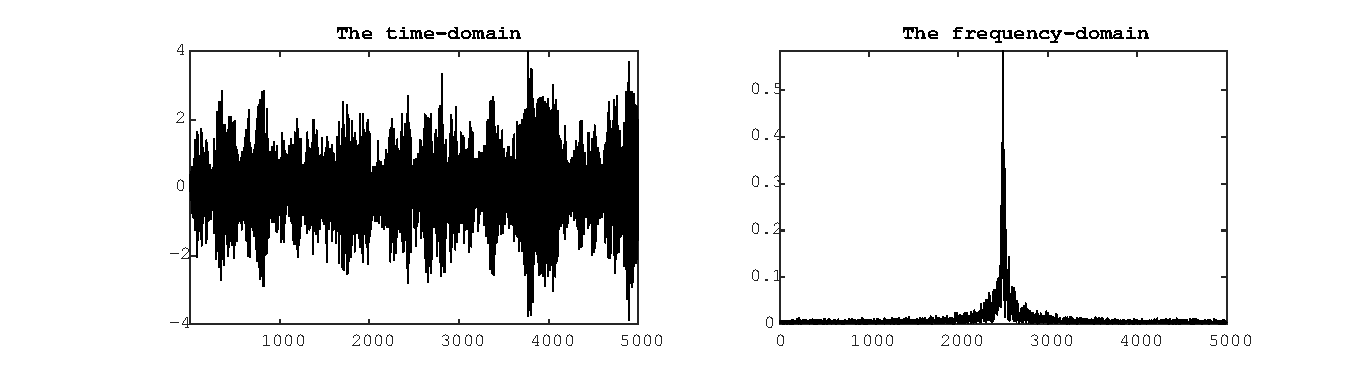
\includegraphics[scale=0.66]{img/fig02.eps}\\
\end{figure}

We can figure out from the graph that $f_c = 2500\hertz$.

\subsection{Estimate the DoA}
The MUSIC algorithm is implemented through MATLAB:
\lstinputlisting[
    language = Matlab, 
    caption = {\bf narrowband.m},
    label = {../src/narrowband.m}
]{../src/narrowband.m}

The result of the algorithm is:

\begin{figure}[H]
    \centering 
    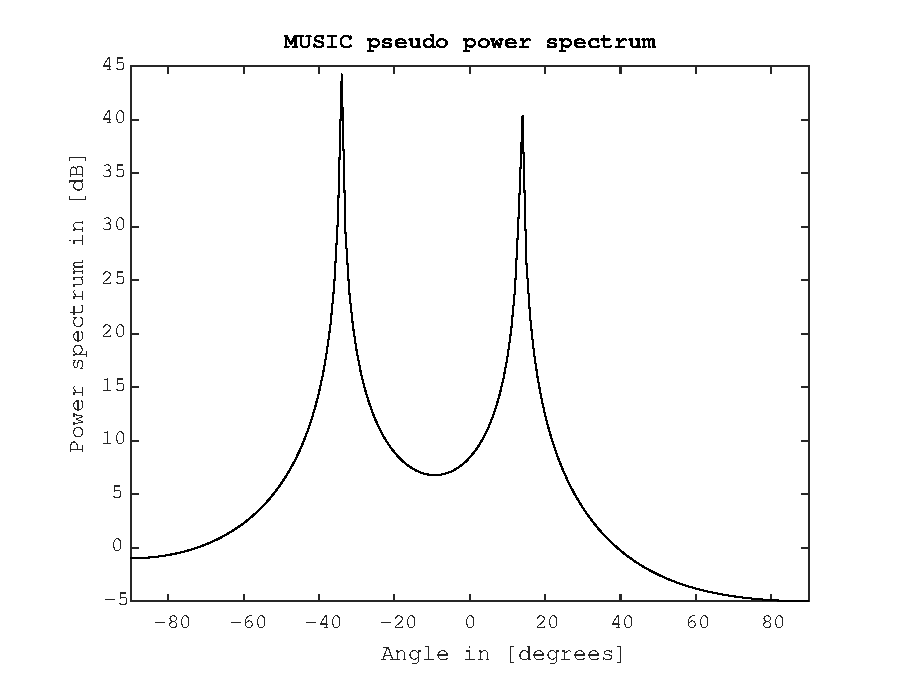
\includegraphics[scale=0.5]{img/fig01.eps}\\
\end{figure}

Which claims that:
\begin{lstlisting}
    The desired source DOA with MUSIC is: -14 deg
    The interfering DOA with MUSIC is: 34 deg
\end{lstlisting}

\section{Broadband Estimation}
\hspace{0.5em} Since broadband speech signal can be non-stationary, we need STFT(Short-time Fourier Transform) to keep information on frequency domain and time domain at the same time.

The ISSM(Incoherent Signal Subspace Method), which perform STFT on the original signal, and do MUSIC with its result in row. We've read the original paper of ISSM, and ... Whatever, here I'm going to prove the map between frequency and the index in FFT.

In MATLAB, function FFT will perform
\begin{gather}
    Y[k] = \sum_{j = 1}^{n}{X[j]}e^{-i 2\pi(j - 1)(k - 1)/n}
\end{gather}

Thus, in case that the original signal $X[j] = e^{i 2 \pi f \cdot (j - 1) / f_s}$, 
\begin{gather*}
    Y[k] = \sum_{j = 1}^{n}{e^{i 2 \pi (j - 1)\big[\frac{f}{f_s} - \frac{k - 1}{n}\big]}}
\end{gather*}
The modulus of the result can reach its peak when k equals to some number. Let $u = \frac{f}{f_s} - \frac{k - 1}{n}$, using Euler's formula to transform it into $(u \neq 0)$
\begin{gather*}
    \mathrm{Re}\{ Y[k] \} = \sum_{j = 1}^n{\cos[ 2 \pi u \cdot (j - 1)]} = \frac{1}{2}(\csc(\pi \cdot u) \sin[(2n - 1)\pi \cdot u] + 1) \\
\mathrm{Im}\{ Y[k] \} = \sum_{j = 1}^n{\sin[ 2 \pi u \cdot (j - 1)]} = \frac{1}{2}\csc(\pi \cdot u)(\cos(\pi \cdot u) - \cos[(2n - 1)\pi \cdot u])
\end{gather*}
Consider the graph of $\csc$ function, and other $\sin$ or $\cos$ part limit it with an approximated 1 value, when u approach to 0, the modulus grows up quickly. And when $u = 0$, as $Y[k] = n$
\begin{gather}
    \frac{f}{f_s} = \frac{k - 1}{n} \Rightarrow f = \frac{(k - 1)f_s}{n}
\end{gather}

\subsection{Plot the wave and frequency response}
The figure:
\begin{figure}[H]
    \centering 
    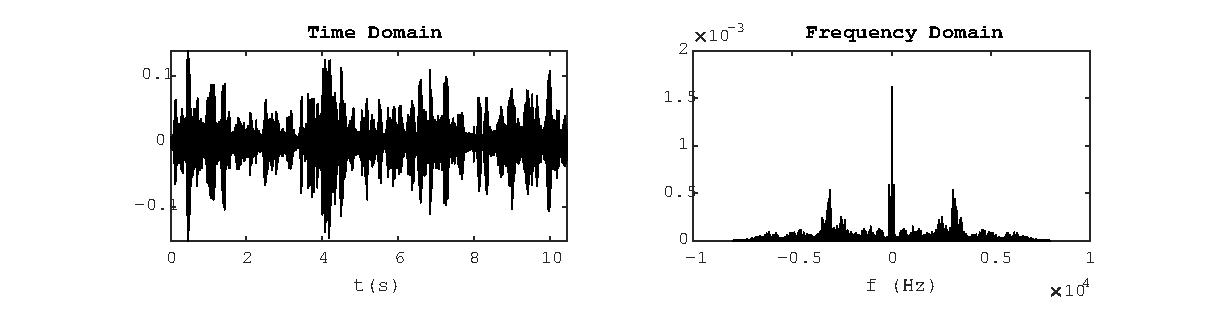
\includegraphics[scale=0.7]{img/fig03.eps}\\
\end{figure}
Its easy to figure out that the frequency covers a wide span of frequency and can not find a $f_c$.

\subsection{Perform STFT and MUSIC with spectral density matrix}
\hspace{0.5em} The processes of ISSM are
\begin{enumerate}
    \item Perform STFT on the original signal matrix.
    \item Perform MUSIC with some of its frequency span.
    \item Add them together, get the result.
\end{enumerate}

The ISSM algorithm is implemented through MATLAB:

\lstinputlisting[
    language = Matlab, 
    caption = {\bf broadband.m},
    label = {../src/broadband.m}
]{../src/broadband.m}

The result of the algorithm is(STFT Para: [len = 512/inc = 512]):

\begin{figure}[H]
    \centering
    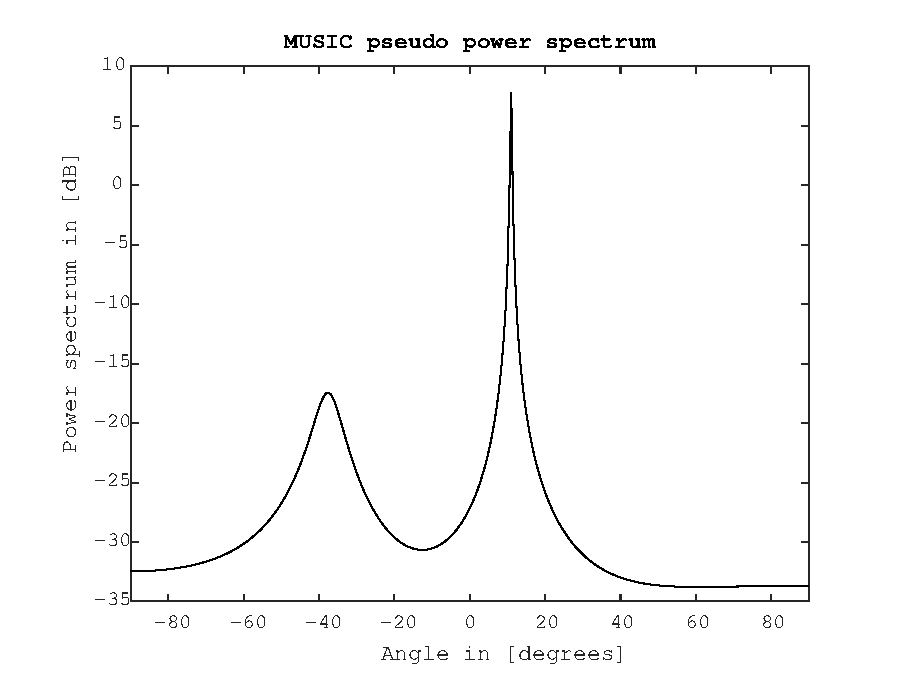
\includegraphics[scale=0.7]{img/fig04.eps} \\
\end{figure}

Which claims that:
\begin{lstlisting}
    The first source with MUSIC is: -38 deg
    The second source with MUSIC is: 11 deg
\end{lstlisting}

\newpage
\section{Microphone Array Experiment(with bonus)}
\subsection{Adjustment}
\hspace{0.5em} Real time circumstance is rather complex than the stimulation data, so there's more special cases to deal with. For example, if the result have a long vacant span, there will be a high peak in $deg = 0$ which will interfer our result.

% \begin{figure}[H]
%     \centering
%     \includegraphics[scale=0.6]{img/fig05.eps} \\
% \end{figure}

There're multiple solutions to the problem, we can fillter the low frequency band $[0, 20]$ to mitigate the impact of vacant span. Or we can filter the result with its power spectrum. In a word, there's ways through time domain and frequency domain to solve the problem. We chose the former method.


\end{document}